\chapter{SYSTEM DEVELOPMENT METHODOLOGY}
\section{Introduction}This chapter walks through the methodology behind building LexiFlow and how it kept the whole stuff on track. It kicks off by explaining why we went with a hybrid Agile model. Basically, we borrowed bits from both Agile and traditional project management, since that gave us flexibility without losing structure, and we held onto fixed development milestones to stay grounded. So each phase of the approach gets its own discussion here. The result is a full picture of how the project moved along, right from gathering those first requirements all the way to testing and finally deploying the system. The methodology section also digs into how the technologies we picked truthfully fit into the Agile workflow and line up with what LexiFlow needs. The chosen tools and the features they bring had to mesh with the way we worked. And that's the point. The whole stack was meant to back up what the application truthfully does.
\section{Methodology Choice and Justification}We went with a hybrid Agile model for LexiFlow since it bends easily when requirements shift, yet still keeps the milestones structured. It lets development happen in iterations, so feedback and tweaks keep flowing through the whole project. Agile fits software work like this honestly well, where user needs tend to revamp over time, since it leans on collaboration, keeping the customer involved, and rolling with change as it comes. Scrum can sharpen communication, cooperation, and the quality of the product itself, based on what~\citet{scrum}. Waterfall, on the flip side, lines the phases up in order, which helps new developers really get a feel for the `big picture`of running a software project across its life cycle. That ordering also gives them a deeper handle on the requirements, the code logic, and how testing works. Every phase here leans on Agile basics, regular sprints, user stories, continuous integration. You get fast prototyping and feature testing this way, which keeps the end product actually matching what users want. {As figure {\ref{fig:methodology_overview}} shows}, we're also folding in traditional practices like detailed planning and documentation, so nothing about the system slips through the cracks (interestingly). \begin{figure}[ht]
    \centering
    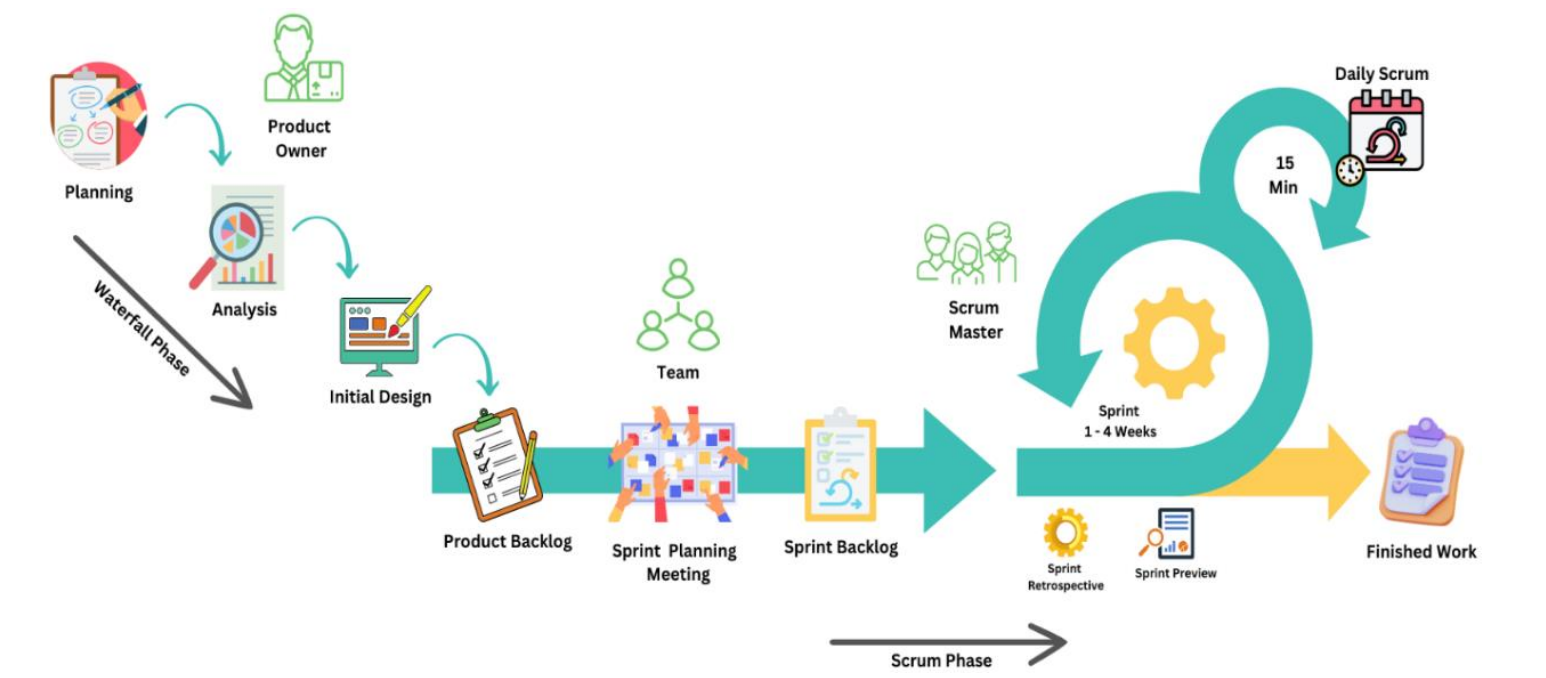
\includegraphics[width=1\textwidth]{./figs/scrum2.png}
    \caption{Hybrid-Scrum Methodology Overview~\citep{scrum2}}
    \smallskip
    \label{fig:methodology_overview}
\end{figure}
\section{Methodology Phases}building LexiFlow will follow a hybrid methodology consisting of several key phases:
\begin{enumerate}[label= (\alph*)] \item \textbf{Planning (Waterfall):} This phase sets up everything that follows. It covers preliminary scoping, time estimates, who gets assigned what, and figuring out the key stakeholders. The whole piece leans on a traditional Waterfall approach, where you map out the entire roadmap upfront so the project's got a clear direction right from the get going \item \textbf{Analysis (Waterfall):} Here's where every requirement gets carefully pulled apart and written down, again using Waterfall. The process pulls in everyone involved. Language learners and lecturers go through a thorough interview or survey, and the idea is to make a genuine attempt at nailing down every functional and non-functional requirement there is. \item \textbf{Initial Design (Waterfall):} Once the requirements are locked in, the project moves straight into design, even so Waterfall. This step builds a high-level strategy for the whole system, and it spells out how each component talks to the others through its interfaces. By keeping the design closely tied to what users actually asked for, we create sure every piece is clearly defined and ready to head into development. \item \textbf{Actual Sprints (Agile):} Development runs across six sprints: \begin{enumerate}[label= (\roman*)] \item \textit{Sprint 1, Prototype Sprint:} An early prototype covering the core functions gets built. The point is to check those early design assumptions, gather feedback, and see how well the chosen models really perform. \item \textit{Sprint 2, User Module:} This one's all about user registration, login, and profile management. Both students and lecturers can create accounts, manage them, and set their learning preferences. \item \textit{Sprint 3, Content Processing Module:} During this sprint we build the local media uploading and YouTube URL submission features. The system processes the content and spits out synchronized subtitles in Mandarin, pinyin, and English translation. \item \textit{Sprint 4, Interactive Learning Module:} This sprint handles the vocabulary side of things, stuff like word search, saving vocabulary, bookmarking video segments, and flagging translation errors so the content stays accurate. \item \textit{Sprint 5, Assessment Module:} This sprint brings in the review and testing features. It includes generating flashcards from saved vocabulary and auto-creating quizzes based on the user's learning history.
\item \textit{Sprint 6, Deployment Sprint:} This is where everything comes together. All modules go through final integration and testing, and then the system gets deployed to the live environment with final checks, performance tweaks, and the documentation wrapped up. \item \textbf{Burn Down Chart (Agile):} A burn down chart gets kept up throughout each sprint to track the work that's left against the time available. It's a visual that lets the team check progress every day, spot bottlenecks quick and confirm the sprint's still heading toward its goals. It also comes in handy as a reference objective during the Sprint Review. \item \textbf{Sprint Review (Agile):} Once a sprint wraps, there's a review session where the new features get shown off to stakeholders. Whatever feedback they give is collected and folded into the goals for the next sprint, which keeps things lined up with what users actually want. \item \textbf{Sprint Retrospective (Agile):} After each sprint review, the team sits down for a retrospective. They look at what worked, what flopped, and how the process could run smoother next time around. This is really what drives the ongoing improvement and keeps the team working together. \item \textbf{Maintenance (Agile):} After deployment, the system moves into maintenance. Following Agile practices, updates and enhancements roll out in iterative cycles to squash bugs, react to user feedback, and add new features, so the product stays solid and user-focused as time goes on. The Gantt chart in Figure~\ref{fig:jira} lays out the timeline for FYP 1 and the prototype sprint, while Figure~\ref{fig:jira2} covers FYP 2. We built the Gantt chart in Jira, a project management tool that helps track how the project's moving along and keeps the tasks manageable. \begin{figure}[H]
    \centering
    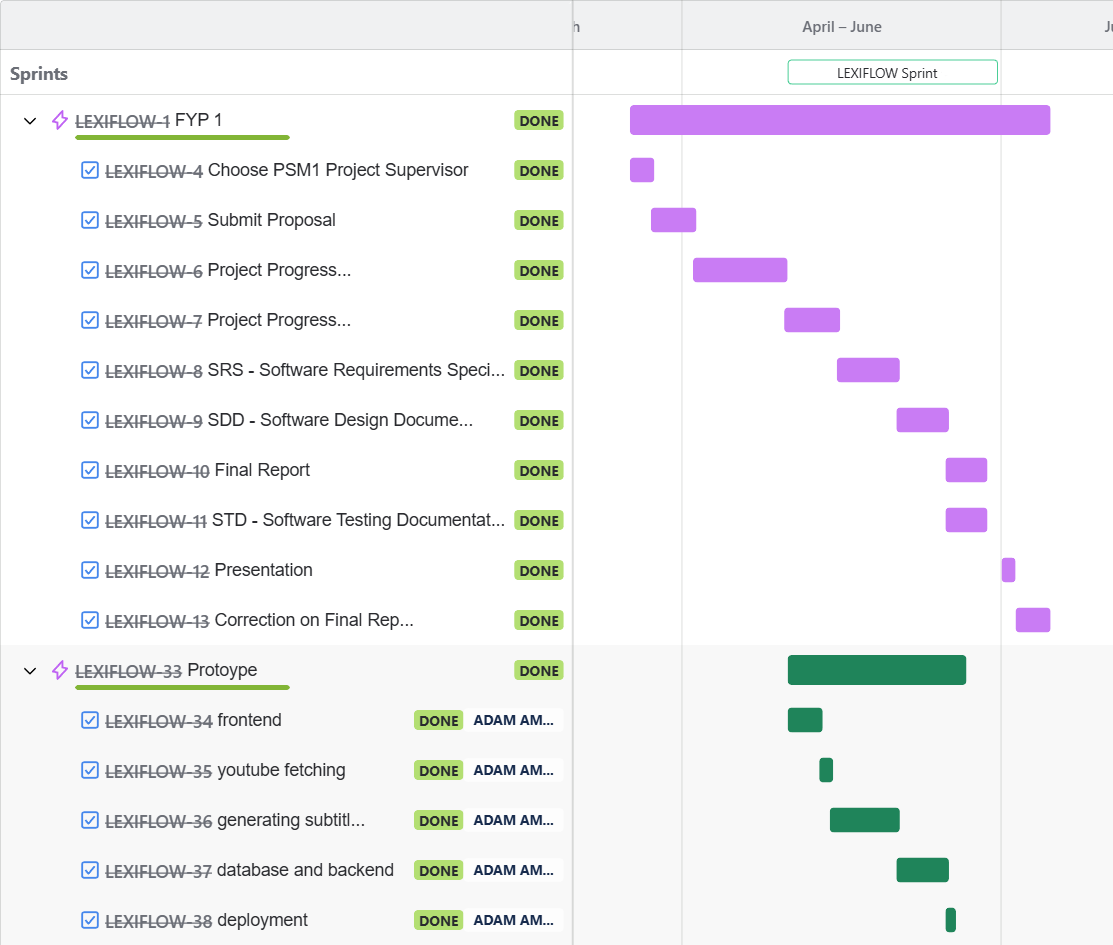
\includegraphics[width=0.75\textwidth]{./figs/fyp1_gantt.png}
    \caption{Gantt Chart FYP1}\label{fig:jira}
\end{figure} \begin{figure}[H]
    \centering
    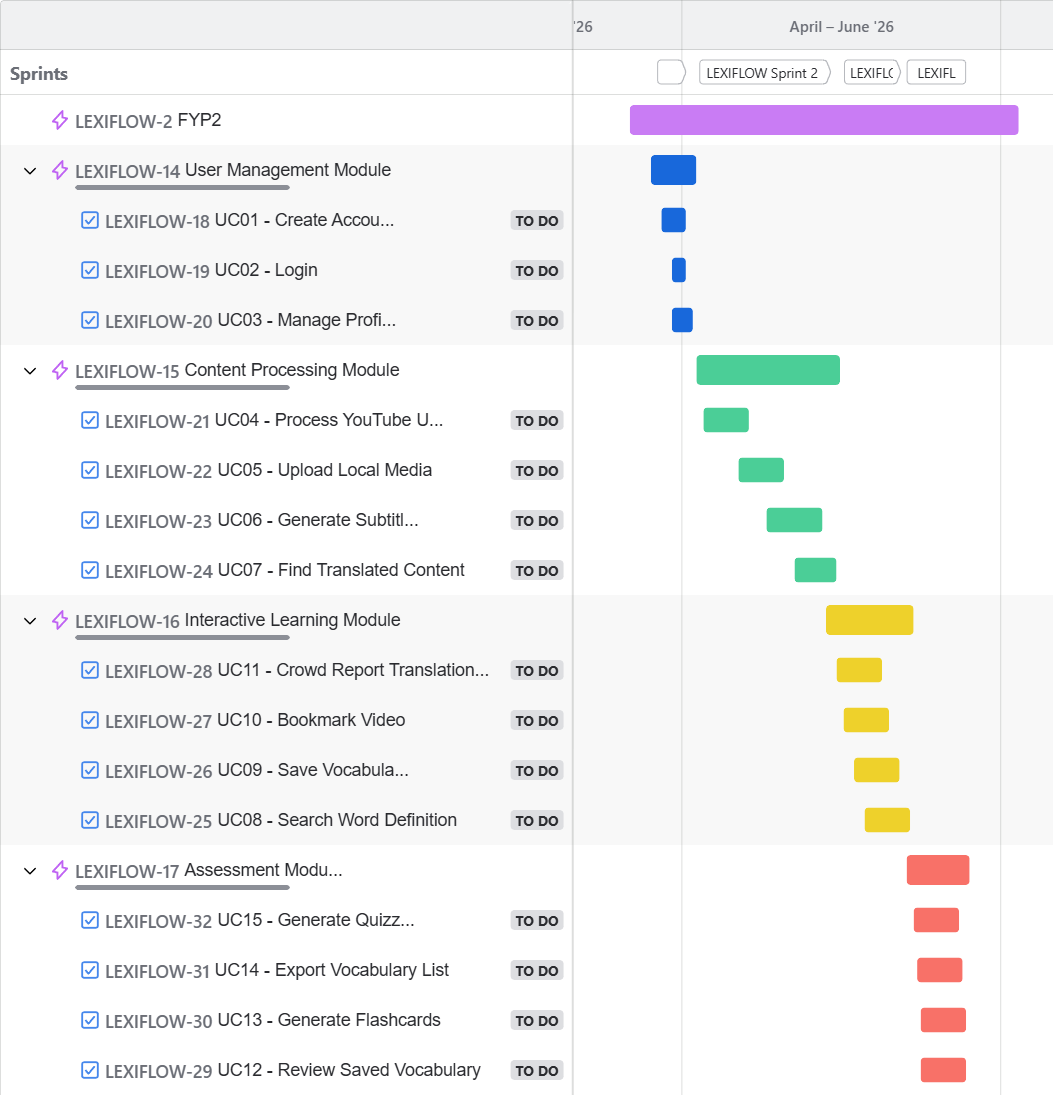
\includegraphics[width=0.75\textwidth]{./figs/fyp2_gantt.png}
    \caption{Gantt Chart FYP2}\label{fig:jira2}
\end{figure} First up is the prototype sprint, which is already done. You can see its burn down chart in Figure~\ref{fig:burndown}. It shows where the project stands and which tasks are still left to finish. The sprint review with the stakeholders is also wrapped up. Their feedback shows up in Appendix~\ref{app:feedback-on-prototype}. \begin{figure}[H]
    \centering
    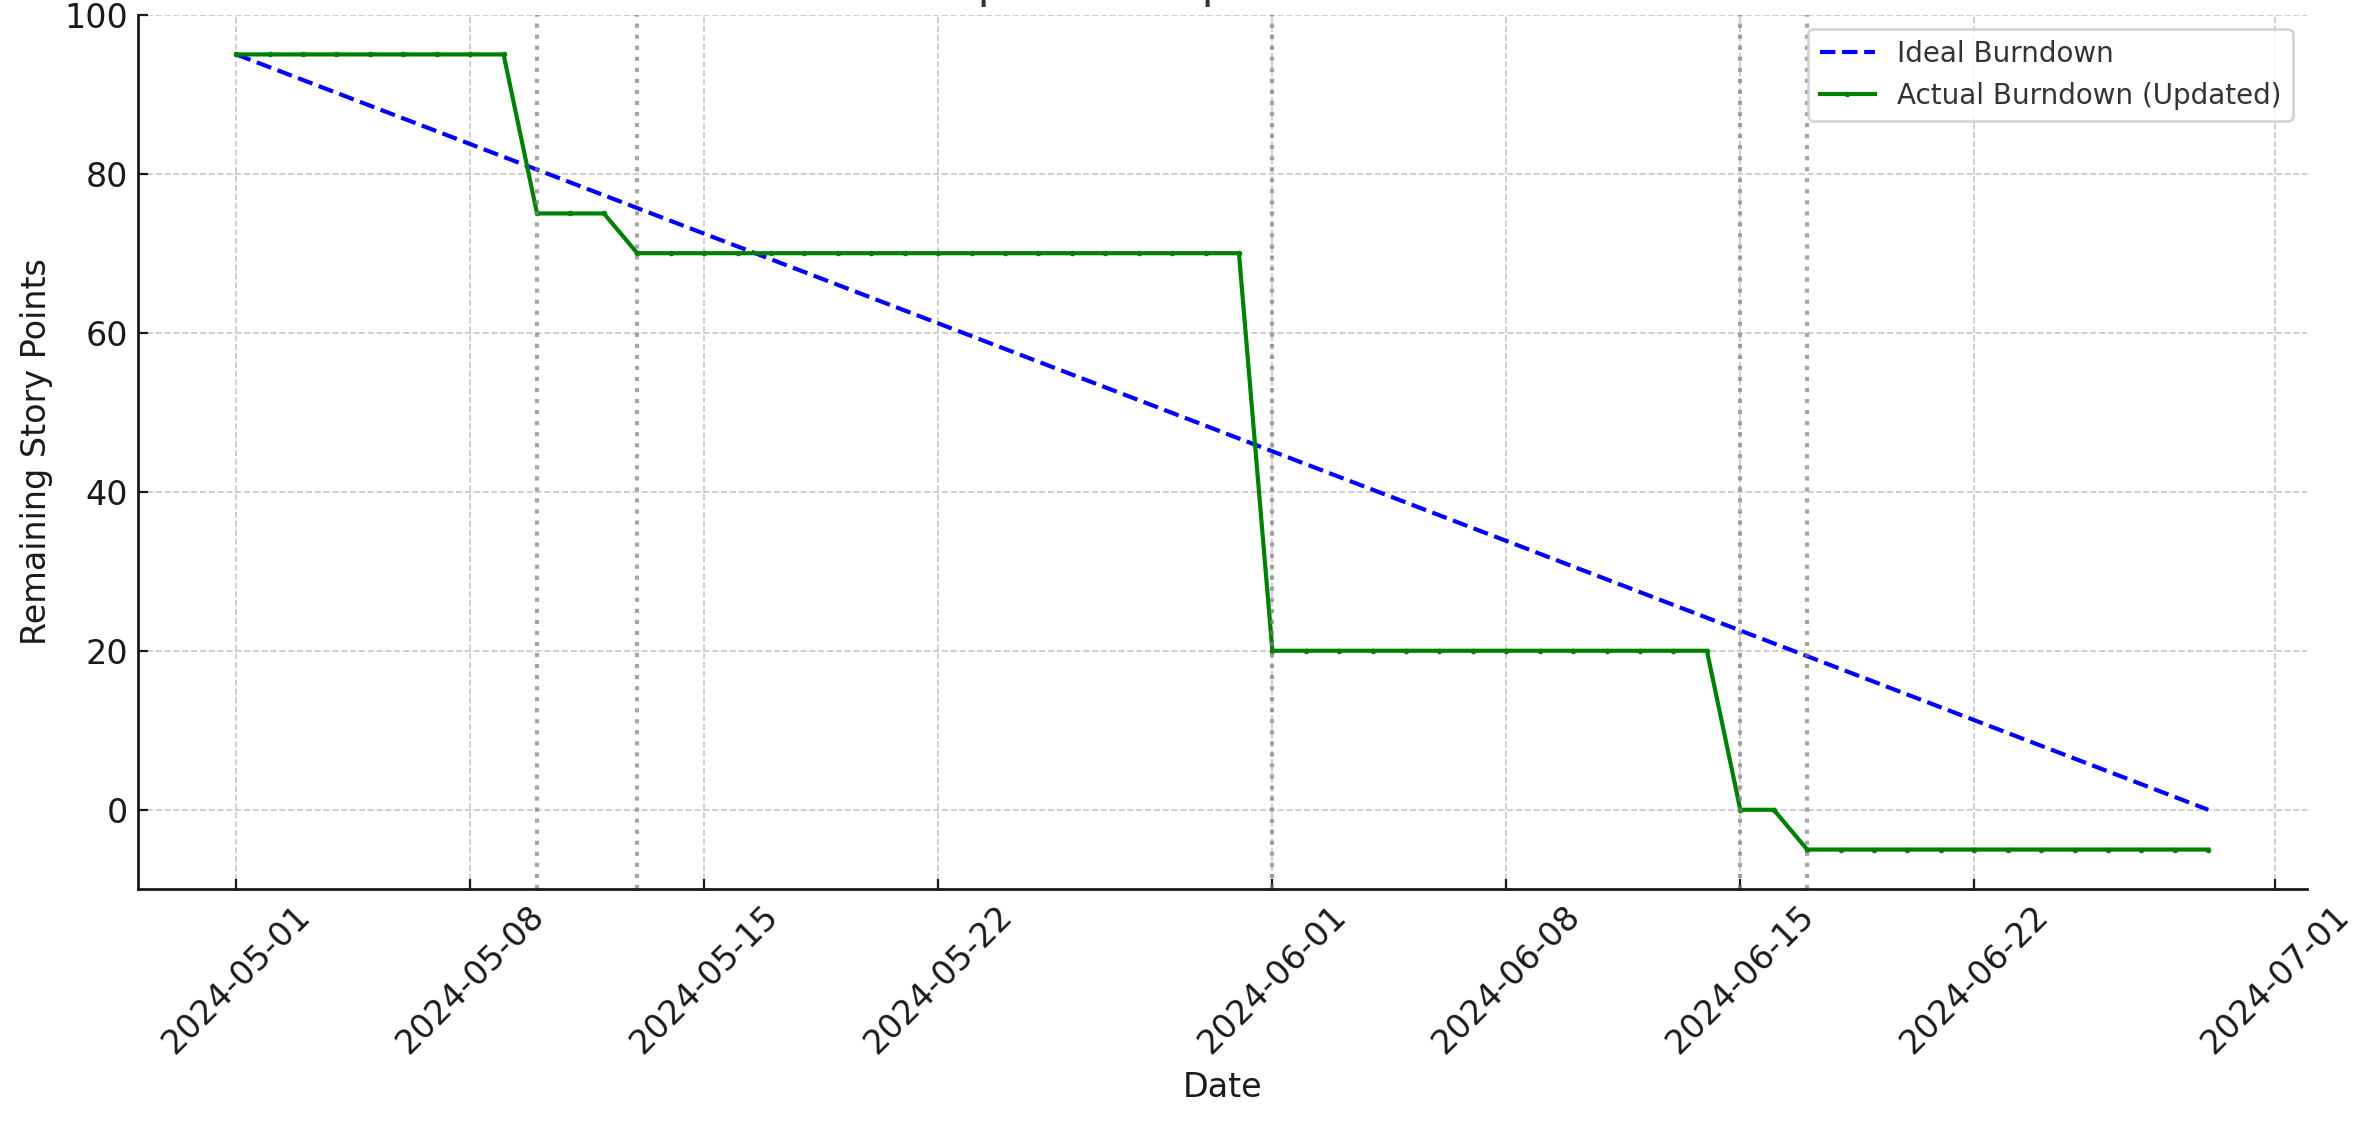
\includegraphics[width=0.8\textwidth]{./figs/burndown.png}
    \caption{Burn Down Chart for Sprint 1 (Prototype)}\label{fig:burndown}
\end{figure}
\section{Technology Stack}This section covers the tech we used to build LexiFlow.
\begin{enumerate}[label= (\alph*)] \item \textbf{Vue.js:} A JavaScript framework for building user interfaces. We picked Vue.js because of its reactive, compiler-improved rendering. It's what we'll use to put together the frontend of the web app. \item \textbf{Node.js:} a JavaScript runtime built on Chrome's V8 engine. We went with it for the non-blocking, event-driven setup, which makes it a solid fit for scalable network apps. It'll handle server-side logic and manage user requests. Basically, it's the control center of our backend, taking requests from the frontend and coordinating with the database and the python microservices. \item \textbf{MongoDB:} A NoSQL database that keeps data in flexible JSON-style documents. We chose MongoDB for its straightforward document model, which pairs unique objects with their own documents and makes data management a lot simpler. That's precisely what we aim for for storing user-generated material, audio/video metadata, and the processed subtitles. \item \textbf{FastApi:} A modern, fast web framework that's meant to make building APIs in Python easier, using standard Python type hints. We picked FastAPI for how easy it is to labor with and that it generates documentation automatically. The backend services will use it to turn our python scripts into RESTful APIs, so our Node.js server can talk to the services that take care of audio processing, transcription, and translation. \item \textbf{SileroVAD:} Silero VAD does a great job across audio from all sorts of domains, with different background noise and quality levels. It was trained on a huge dataset covering over 6000 languages. We chose it for its accuracy and how easy it is to use. It'll detect speech segments and break them into sentence-level chunks. \item \textbf{Whisper:} a powerful automated speech recognition system trained on a varied set of multilingual speech data. We went with it for its accuracy and its knack for handling all kinds of languages and accents. It'll transcribe the audio into text, giving us the base for everything that comes next. \item \textbf{painlessM4Tv2:} Meta's multilingual, multimodal machine translation model, which we'll use to translate Mandarin text into English. We chose it for its high-quality translation across plenty of languages, Mandarin and English included. \item \textbf{PyPinyin:} A Python library that converts Chinese characters to pinyin. We'll use PyPinyin to provide users pronunciation help for Mandarin text, making the whole thing easier to learn.
LexiFlow leans on automated workflows to keep updates running smoothly. As Figure~\ref{fig:ci_cd} shows, developers commit their code changes to Git first, which handles version control. From there, GitHub Actions builds and tests everything on its own. Then Docker packages the working app so Nginx can deploy it. The nice piece This pipeline catches bugs early and keeps releases stable. You can see in the figure how all these steps tie back to our planning and monitoring, which keeps things efficient. It fits our hybrid Agile approach too, frequent updates, but the system stays steady (in my view). \begin{figure}[H]
    \centering
    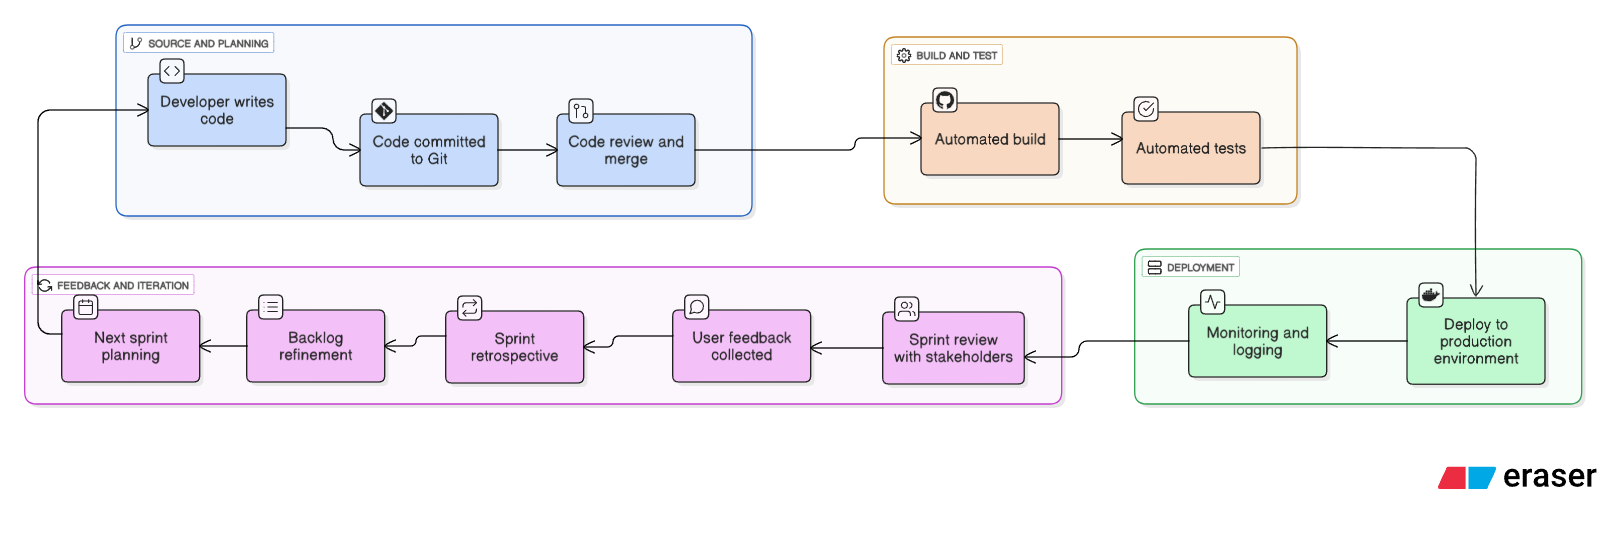
\includegraphics[width=1\textwidth]{./figs/ci_cd.png}
    \caption{CI/CD Pipeline for LexiFlow}\label{fig:ci_cd}
\end{figure}
\section{System Requirement Analysis}This section lays out the system requirements, hardware, software, all of it. Honestly, these details matter when you're trying to hit the functional and performance targets. That's basically what keeps development and operation running smoothly for the system we described earlier (if you think about it).
\subsection{Hardware Requirements}To get LexiFlow running smoothly and keep users happy, here's the hardware you'll want in place:
\begin{enumerate}[label= (\alph*)] \item \textbf{Server:} You'll need a dedicated server packing at least 16 GB of RAM, 8 CPU cores, and 500 GB of SSD storage to deal with backend processing, the database, and all those API requests. A GPU with 8 GB of VRAM minimum is a must too, since it handles audio efficiently, especially stuff like speech recognition and machine translation. \item \textbf{Development Machines:} For dev environments, testing frameworks, and local databases, these machines should have 8 GB of RAM at minimum, adequate storage (256 GB SSD or more), and a modern multi-core processor. \item \textbf{Client Devices:} Users just need a device with at least 4 GB of RAM and a current web browser. Chrome, Firefox, Safari, whatever. That's enough to labor with the LexiFlow web app.
\subsection{Software Requirements}LexiFlow needs these software pieces to run:
\begin{enumerate}[label= (\alph*)] \item \textbf{Operating System:} A Linux-based OS (something like Ubuntu 22.04 or newer) for the server side, which keeps things stable and performing well. \item \textbf{Web Server:} Nginx handles the HTTP requests and serves up the LexiFlow web app. \item \textbf{Database:} MongoDB stores user data, audio/video metadata, and the processed subtitles. \item \textbf{Version Control:} Git tracks code changes and manages versions. \item \textbf{Network Protocols:} SSH for secure remote access to the server. \item \textbf{IDE:} Visual Studio Code, which gives you code completion, debugging, and version control built right in. \item \textbf{Visual Design Tools:} Enterprise Architect for the system architecture and UML diagrams. Figma to mock up the user interface (at least that's the plan
\section{Chapter Summary}This chapter walks through how LexiFlow approached things, with a real zero in on the hybrid Agile setup that mixes iterative development with structured phases. So the project could shift when needs changed, but nevertheless hit its milestone checks. We've also gone through the tech stack in detail, explaining the reasoning behind each call. And finally, the hardware and software requirements get laid out here too, which sets things up nicely for a smooth build in the phases that follow.
